\chapter{BOOTSTRAPPING PRIVATE OVERLAYS}
\label{chap:bootstrapping}

While P2P overlays provide a scalable, resilient, and self-configuring platform
for distributed applications, their adoption rate for use across the Internet
has been slow outside of large-scale systems, such as data distribution and
communication.  General use of decentralized, P2P (peer-to-peer) applications
targeting homes and small/medium businesses (SMBs) has been limited in large
part due to difficulty in decentralized discovery of P2P systems, the bootstrap
problem, further inhibited by constrained network conditions due to firewalls
and NATs (network address translators).  While these environments could benefit
from P2P, many of these users lack the resources or expertise necessary to
bootstrap private\footnote{In the context of this chapter, private implies that
the overlay's purpose is not for general use. Once established, such overlays
can support privacy in communication; however, overlay security is beyond the
scope of this chapter and covered in more depth in
Chapter~\ref{chap:security}.} P2P overlays particularly when the membership is
unsteady and distributed across wide-area network environments where a
significant amount of (or all) peers may be unable to initiate direct
communication with each other due to firewalls and NAT (network address
translation).

Examples of large-scale P2P systems include Skype, BitTorrent, and Gnutella.
Skype is a voice over P2P system, whereas BitTorrent and Gnutella are used for
file sharing.  The bootstrapping in these systems typically relies on overlay
maintainers using high availability systems for bootstrapping, bundling their
connection information with the application distribution.  The application then
uses theses servers during the initialization phase to connect with other peers
in the system.  Alternatively, some services constantly crawl the network and
place peer lists on dedicated web sites. A new peer wishing to join the network
queries the web site and then attempts to connect to the peers on this list.

In smaller-scale systems, P2P interests focus on decentralization.  For
example, users may desire to run an application at many distributed sites, but
the application lacks dedicated central servers to provide discovery or
rendezvous service for peers.  In contrast, dedicated, centralized P2P service
providers, such as LogMeIn's Hamachi, a P2P VPN (virtual private network), may
collect usage data, which the users may wish to remain private, or are not free
for use.

Many applications make sense for small-scale overlay usage, including
multiplayer games, especially those that lack dedicated online services;
private data sharing; and distributed file systems.  Clearly, a small P2P
system could be bootstrapped by one or more users of the system running on
public addresses, distributing addresses out-of-band, instructing their peers
to add that address to their P2P application, and then initiate bootstrapping;
but these types of situations are an exception and not the norm.  Ultimately,
the users would be enhanced significantly through approaches that can make
decentralized bootstrapping transparent through minimal and intuitive
interaction with the P2P component.

\begin{figure}
\centering
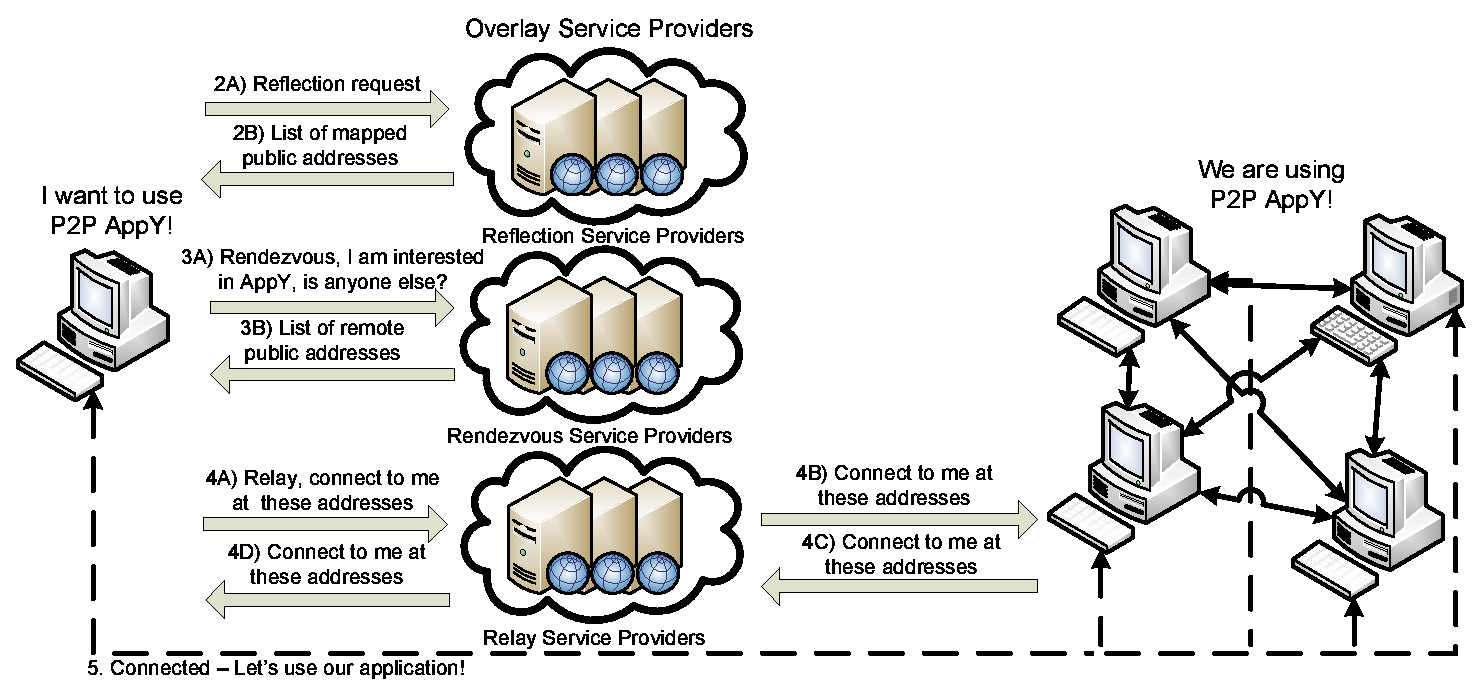
\epsfig{file=figs/bootstrap.eps, width=5.5in}
\caption{Bootstrapping a P2P system using an existing (generic) overlay.}
\label{fig:bootstrap}
\end{figure}

The basic bootstrapping process can be broken down into two components: finding
and connecting to an active peer in the system.  When a node starts, it
contacts various bootstrap servers, until it successfully connects with one,
upon which they exchange information.  The bootstrap server may inquire into
the overlay for the best set of peers for the new peer and respond with that
information or it may respond with its existing neighbor set.  At which point,
the peer attempts to connect with those peers.  This process continues
aggressively until the peer arrives at a steady state, either connecting with a
specific set of or a number of peers.  Afterwards, the P2P logic becomes
passive, only reacting to churn from new incoming or outgoing peers.

Overlay support for constrained peers, i.e., those behind NATs and restrictive
firewalls, requires additional features to support all-to-all connectivity for
peers in the overlay.  The instantiation of P2P systems for private use could
become overly burdensome, potentially relying on significant human interaction
to bootstrap them, for example, by relaying connection information through
phone calls and e-mail.  Even if this is feasible, this sort of interaction is
undesirable.  P2P systems should be self-discovering, minimizing the amount of
work users need to do in order to take advantage of them, a feature stressed by
ad-hoc systems.  In addition, these approaches may rely on centralized
components; if they become unavailable, which is a possibility since most users
lack the expertise in configuring highly available systems, the system will not
be accessible.

To address this, I have explored the possibility of using existing public
overlays as a means to bootstrap private overlays.  There are many existing
public overlays with high availability, such as Skype, Gnutella, XMPP
(Extensible Messaging and Presence Protocol), and BitTorrent; by leveraging
these systems, system integrators can easily enable users to seamlessly
bootstrap their own private P2P systems.  In the preceding paragraphs, I have
identified the components necessary for bootstrapping a homogeneous system; in
the following, I will expand them for environments to support the bootstrapping
of a private overlay from a public overlay with consideration for network
constrained peers.  The public overlay must support the following mechanisms as
illustrated in Figure~\ref{fig:bootstrap}:

\begin{itemize}

\item {\bf Reflection}. A method for obtaining global application and IP
addresses or identifier for a peer that can be shared with others to enable
direct communication.

\item {\bf Relaying}. A method for peers to exchange arbitrary data, when a
direct IP link is unavailable.

\item {\bf Rendezvous}. A method for identifying peers interested in the same
P2P service.

\end{itemize}

This work motivates from the belief that while small-scale P2P systems are
attractive for decentralized systems, the overheads relating to creating and
maintaining bootstrap services make them unfeasible.  A public overlay can be
used to transparently bootstrap a private overlay with minimal user
interaction.

The requirements are presented and verified in the context of two prototype
implementations: a XMPP / Jabber~\cite{xmpp} and Brunet~\cite{brunet}.
XMPP-based overlays are commonly used as chat portals, such as GoogleTalk and
Facebook Chat.  XMPP also supports an overlay amongst servers forming through
the XMPP Federation, which allows inter-domain communication amongst chat
peers, so that users from various XMPP servers can communicate with each other.
Brunet provides generic P2P abstractions as well as an implementation of the
Symphony structured overlay.  I present the architecture for these systems, the
lessons learned in constructing and evaluating them, and provide an analysis of
the latency to establish peer connectivity in a small-scale private Brunet
overlay with NAT-constrained nodes.

The organization of this chapter follows.  Section~\ref{bs:background}
overviews existing solutions to the bootstrapping problem, and NAT challenges
in P2P systems.  Section~\ref{bs:overview} presents a survey of overlays,
applying the requirements for private overlay bootstrapping to them, and then
show in detail how they can be applied to Brunet and XMPP.  My implementation
is described in Section~\ref{bs:implementation}.  In
Section~\ref{bs:evaluations}, I perform a timing evaluation of bootstrapping
overlays using my prototype on PlanetLab and discuss experiences in deploying
the system.  

\section{Current Bootstrap Solutions}
\label{bs:background}

As described in the introduction, the simple case of bootstrapping is limited
to one peer attempting to find an active peer in the overlay in order for
itself to become a member.  The large-scale providers have resources not
readily available to small-scale overlays.  This section reviews existing
techniques and those being developed and describes their application to
small-scale systems.

When using dedicated bootstrap overlays, a service provider hosts one or more
bootstrap resources.  Peers desiring to join the overlay query bootstrap nodes,
until a successful connection is made to one.  The bootstrap server will then
assist in connecting the peer to other nodes in the P2P system.  Bootstrap
nodes are either packaged with the application at distribution time or through
a meta data file, such as in BitTorrent.  Drawbacks to this approach for small,
ad-hoc pools include that the same server would have to be used every time to
bootstrap the system, or users would have to reconfigure their software to
connect to new bootstrap servers over time; at least one peer must have a
publicly accessible address; and a bootstrap server can become a single point
of failure.

Another commonly used approach for large-scale systems is the use of a host
cache~\cite{host_cache}.  Clients post current connection information to
dedicated web services, a host cache, that in turn communicate with other host
caches.  For small, ad-hoc networks, a host cache acts no differently than a
centralized rendezvous point, requiring that at least one peer has a publicly
accessible address.

``P2P VPN's''~\cite{p2pvpn} use of a BitTorrent tracker is similar to the host
cache concept.  The tracker hosts file meta data and peers involved in sharing.
For the VPN, the peer registers a virtual file used to organize the peers, a
form of rendezvous.  Each peer in the VPN queries the tracker regarding the
file, registers its IP address, and receives other active ``sharers'' IP
addresses.  Peers on public addresses or using UPnP (universal plug and play)
are able to receive incoming connections from all other peers.  The problem
with this approach is that it is heavily user-driven.  A user must register
with each BitTorrent tracker individually and maintain a connection with each
of them, in order to handle cases where BitTorrent trackers go offline.  In
addition, this does not use the BitTorrent trackers in a normal fashion, so it
may be banned by tracker hosts.

Research has shown that peers can use the locality properties of recent IP
(Internet Protocol) addresses in a large-scale P2P system to make intelligent
guesses about other peers in the P2P system using an approach called random
probing~\cite{bootstrapping_p2p, locality_aware}.  The results show that, in a
network of tens to hundreds of thousands of peers, a bootstrapping peer can
find an active peer in 100 guesses to 2,000 guesses, depending on the overlay.
The approach does not really apply well to small-scale systems, especially when
peers are constrained by NATs and firewalls.

Rather than distribute an IP address, which points explicitly to some location
in the Internet, a small P2P network can apply a name abstraction around one
peer in the overlay using Dynamic DNS~\cite{bootstrapping_ddns} (domain name
service).  Peers share a DNS entry, which points to a bootstrap server.  When
the peers detect that the bootstrap server is offline, at random time intervals
they will update the DNS entry with their own.  The application of this
approach is well-suited to small, ad-hoc groups, as the service could be
distributed across multiple Dynamic DNS registrations.  However, sharing a DNS
entry requires trusting all peers in the overlay, making it easy for malicious
peers to inhibit system bootstrapping.  Also the approach requires that at
least one peer be publicly addressable; if a non-publicly addressable peer
updates the cache inadvertently, it could delay or permanently prevent peers
from creating a P2P system.  The reported results~\cite{bootstrapping_ddns}
were simulation-based and did not determine how well a dynamic DNS handles
rapid changing of name to IP mappings.

IP supports multicasting to groups interested in a common service.  In the case
of bootstrapping a P2P system~\cite{pastry, locality_aware}, all peers would be
members of a specific group.  When a new peer comes online, it queries the
group for connection information and connects to those that respond.  The
approach, by itself, requires that all peers are located in a multicast capable
network, restricting this approach typically to local area networks.

A large-scale structured overlay~\cite{one_ring, p2p_bootstrap} could enable
peers to publish their information into a dedicated location for their service
or application and then query that list to obtain a list of online peers.
Peers could search for other peers in their overlay and connect with them using
their connection information.  Since the service would be a large-scale system,
it could easily be bootstrapped by a dedicated bootstrap or host caches.  As it
stands, the described works were position papers and the systems have not been
fully fleshed out.  The primary challenge in relationship to small, ad-hoc
networks is that it lacks details bootstrapping of peers behind NATs into
overlays as it provides only a means for rendezvous and not reflection nor
relaying.

\section{Core Requirements}
\label{bs:overview}

As presented in the preceding sections, a solution to bootstrapping small P2P
overlays must address several challenges, namely reflection, rendezvous, and
relaying.  This section presents a generic solution to this problem.  The basis
for my solution is reusing existing, free-to-join public overlay.  In order to
support these features the public overlay must have mechanisms for peers to
obtain a public network identity (reflection); search for other peers that are
bootstrapping the same P2P service (rendezvous); and send messages to peers
through the overlay (relaying).  These are the minimum requirements to
bootstrap a decentralized, P2P system when all peers are behind NATs.

\subsection{Reflection}
\label{bs:reflection}

Reflection provides a peer with a globally-addressable identifier for receiving
incoming messages from other peers.  Without reflection, peers on different
networks with non-public addresses are unable to communicate directly with each
other.  Reflection is not limited to IP.  For example, when a peer joins a
service, such as a chat application or a P2P system, the overlay provides a
unique identifier, which also serves as a form of reflection.

In IP communication, reflection enables NAT traversal.  The simplest method for
NAT traversal relies on obtaining the public information for an existing UDP
(user datagram protocol) socket and then sharing that with other peers.  This
behavior can be supported through either local service or remote assistance.
The local approach approach relies on having a router with a public IP address
supporting either UPnP~\cite{upnp} or port forwarding / tracking.  In many
cases, UPnP is not enabled by default and in most commercial venues it will
rarely be enabled.  Port forwarding / tracking requires non-trivial router
configuration, outside the comfort range of many individuals and is not uniform
across routers.  A peer using UPnP needs no further services, as UPnP enables a
peer to set and obtain both public IP address and port mappings.  Port
forwarding and tracking mechanisms still require that the user obtains and
inputs into the application their public IP address or use in-band assistance
described next.

In the remotely assisted scenario, a peer first sends a message to a reflection
provider, perhaps using STUN~\cite{stun_rfc} (Simple Traversal of UDP through
NATs).  The response from the provider tells the peer from which IP address and
port the message was sent.  In the case of all cone NATs, this will create a
binding so that the peer can then share that IP address and port with other
peers behind NATs.  When the two peers communicate simultaneously, all types of
cone NATs can be traversed; the timing of messages needs to be carefully
considered, however, since NAT mappings may change over time.  So long as one
peer is behind a cone NAT, NAT traversal using this mechanism is possible.  The
situation becomes complicated when both peers are behind symmetric NATs, or
when either one of them have a firewall preventing UDP communication.

Peers behind symmetric NATs cannot easily communicate with each other, since
there is no relation between remote hosts and ports and local ports.  Further
complicating the matter is that there are various types of symmetric NATs,
having behaviors similar to the various cone NAT types. There does exists
methods to traverse these NATs so long as there is a predictable pattern to
port selection~\cite{ice}.

Unlike UDP, TCP (transmission control packet) NAT traversal is complicated by
the state associated with TCP.  In many systems, the socket API (application
programming interface) can be used to enable a peer to both listen for incoming
connections and form outgoing connections using the same local addressing
information.  This method works for various types of systems though the success
rate on NATs is low, 40\%~\cite{ice-tcp}.  Other mechanisms rely on out-of-band
communication~\cite{pvc}, or use of complicated predictive
models~\cite{tcp-hole-punching}.

\subsection{Relaying}
\label{bs:relay}

NAT traversal services only deal with one aspect of the bootstrap problem:
reflection.  That is, peers are able to obtain a public address for receiving
incoming connections with no means for to exchange addresses with other peers
nor perform a simultaneous open to traverse restrictive NATs.  To address this
issue, many systems incorporate these NAT traversal libraries while using
intermediaries to exchange addresses as a method of relaying.  Another form of
relaying exists when two peers are unable to form direct IP connections with
each other and route data messages between a third-party.

The most common method for relaying in IP is the use of TURN~\cite{turn}
(Traversal Using Relay NAT).  A peer using TURN obtains a public IP address and
port that can be used as a forwarding address.  When a remote peer sends to
this address, the TURN server will forward the response to the peer who has
been allocated that mapping.  The lack of abstraction in TURN makes the system
heavily centralized, making its application in small-scale systems complicated.  

In overlays, peers typically have an abstracted identifier that does not
associate them with a single server enabling more decentralized approaches to
relaying.  When a remote peer sends a message to the identifier, the overlay
should translate the identifier into network level addresses and forward it to
the destination.  Because of this restriction, messages sent by relaying cannot
have expectations more than that of sending a packet by UDP.  In other words, a
packet will either be received in a reasonable amount of time or not at all.
Support for reliability, streaming, and flow control, if necessary, must be
provided in user-space.

Finally, the service should be asynchronous or event driven.  The previous
requirements would allow peers to relay through a message board or even by
posting messages to a DHT.  The problem with these two approaches is that peers
may very well communicate for long periods of time using these services.  That
means the potential for posting large amounts of data to a service that will
retain it and constantly querying the service to determine if an update is
available.  Both of these are highly undesirable and may be viewed as denial of
service or spam attacks.

\subsection{Rendezvous}
\label{bs:rendezvous}

A rendezvous service allows peers to discover the global identifier of peers
interested in the same service.  For any given overlay, a naive approach for
rendezvous is the use of a broadcast query or random probing to determine if
any other peers are using the same service.  This approach is unreasonable,
depending on the size of the bootstrap overlay compared to the destination
overlay, it may be very difficult to find another peer, some or all peers may
be behind NATs and unreachable without assistance, and in the worst case
scenario a malicious attacker could be waiting for bootstrap requests into the
system.

Rather than attempt to make a single unified rendezvous technique, each overlay
style usually provide an efficient means for rendezvous, thus reducing the
network and time overhead of finding another peer.  For example, in the case of
a DHT, peers can use a single DHT key to store multiple values, all of which
would be addresses used to communicate with peers in the overlay.
Alternatively, in a system like BitTorrent, peers could use the same tracker
and become ``seeds'' to the same virtual file.

\section{Implementations}
\label{bs:implementation}

Table~\ref{tab:overlays} reviews various overlays, the majority of which are
high availability, public, free-to-join overlays, though some research only
overlays are included.  From this list, I chose to extend Brunet and XMPP to
support private overlay bootstrapping.  Brunet provides a structured P2P
infrastructure, though lacks an active, large-scale deployment outside of
academic deployment (mine) due to being rooted in an academic project.  XMPP,
on the other hand, has support from a large contigency of private users and
enables connections between friends with routing occurring across a distributed
overlay.

My implementation makes heavy use of the transports incorporated into
Brunet~\cite{brunet}.  The key distinguishing feature of this library is the
abstraction of sending over a communication link as it supports primitives
similar to ``send'' and ``receive'' that enable the ability to create P2P
communication channels over a variety of transports.  In the next sections, I
will describe how I extended Brunet to be self-bootstrapping as well as
extensions to enable bootstrapping from XMPP.

The application of structured overlays as the basis private overlays focuses on
the autonomous, self-managing property of the overlay network rather than the
ability to scale to very large numbers.  This has also been the motivation of
related work which has employed structured overlays in systems in the order of
10s to 100s of nodes.  For example, Amazon's shopping cart runs on
Dynamo~\cite{dynamo} using a ``couple of hundred of nodes'' or less.  Facebook
provides an inbox search system using Cassandra~\cite{cassandra} running on
``600+ cores''.  Structured overlays simplify organization of an overlay and
provide each member a unique identifier abstracted from the underlying network.
As mentioned in the cited works, they provide high availability and autonomic
features that handle churn well.  When used in small networks, most structured
overlays (including Brunet and Pastry) in effect act as $O(1)$ systems,
self-organizing links that establish all-to-all connectivity among peers.
Brunet explicitly supports all-to-all connectivity, though in some cases may
require constrained peers to route through relays.  This can further be ensured
by setting the amount of near connections for the infrastructures, which in
Brunet is configurable at run time.

\subsection{Using Brunet}
\label{bs:brunet_bootstrapping}

Prior to this work, Brunet bootstrapped using a recently online cache of peers
and IP multicast.  Brunet already supports behavior similar to STUN, such that,
with every connection Brunet makes, peers inform each other of their view of
the remote peers network state, a form of passive reflection.  Peers
also generate a unique 160-bit node identifier that can be used in the overlay
as a directly receive packets regardless of the underlay conditions.

In a single overlay, Brunet supports relaying either through the
overlay or pseudo direct connections called ``Tunnels''~\cite{hpdc08_0}, where
peers route to each other through common neighboring connections.  The relaying
in this context is used either to maintain a necessary overlay connection, or
to exchange intentions to connect with each other through ``ConnectToMessage''
messages.  Thus when a peer desires a connection to another, both peers
simultaneously attempt to connect to each other after exchanging endpoints
discovered through reflection using the overlay relay mechanisms, dealing with
the issue of more restrictive cone NATs and the case when the peer is behind a
non-traversable NAT.  

To support relaying within the scope of a private overlay, I have
further extended Brunet's transport library to support treating an existing
overlay as a medium for point-to-point communication. This is called a
``Subring'' transport, because it supports the abstraction of multiple private
sub-rings within a common large structured ring.  When the private overlay
transmits data across the public overlay, the private overlay packet is
encapsulated (and possibly encrypted) in a packet that ensures it will be
delivered to the correct private destination usually by means of greedy routing
on the public overlay.  In order to instruct peers to establish ``Subring''
links, they exchange an identifier of the form ``brunet://P2P\_ID''.

Peers store their ``Subring'' identifiers into the DHT for rendezvous.
The DHT provides a scalable and self-maintaining mechanism for maintaining a
bootstrap, so long as the DHT supports multiple values at the same key, as
Brunet does.  The key used for the DHT rendezvous is a hash of the services
name and its version number, which I call a namespace.  Peers can then query
this entry in the DHT to obtain a list of peers in the private overlay.  Since
DHTs are soft-state, or lease systems, where data is released after a certain
period of time, an online peer must actively maintain its DHT entry.  In the
case that a peer goes offline, the DHT will automatically remove the value
after its lease has expired.

To support reflection in the private overlay, there were two potential paths.
The first would have been to extend Brunet to support STUN in each of the
remote servers and then have a private node query them for their public
information.  The problem with this approach is that it would require
maintaining additional state in order to discern which of the remote peers are
on public addresses and can provide STUN services.

Instead, I opted to multiplex the socket used for the public overlay as it
already had gone through the process of ``reflection''.  The multiplexing of a
single socket for multiple overlay is called ``Pathing''.  In this context, the
public and private overlays are given a virtual transport layer that hooks into
an another transport layer, thus not limited purely to socket transport layers.
When peers exchange identifiers, instead of transmitting a simple identifier
like ``udp://192.168.1.1:15222'', the ``Pathing'' library extends it to
``udp://192.168.1.1:15222/path'', where each path might signify a unique
overlay.

The completed approach is illustrated in Figure~\ref{fig:bootstrap_brunet}.
The approach of ``Subring'' and ``Pathing'' enabled the reuse of the core
components of Brunet.  Using ``Subring'' enables peers to form bootstrap
connections to then exchange ``ConnectToMessage'' messages.  If the direct
connections failed, then the ``Subring'' connections could be used as permanent
connections.  The use of ``Pathing'' meant reuse of existing NAT traversal
techniques and limited the amount of system resources required to run multiple
overlays.  In terms of total lines of code, these abstractions enabled a
recursive overlay bootstrapping with a relatively small code footprint, less
than 1000 lines of code.

\begin{center}
\begin{figure}
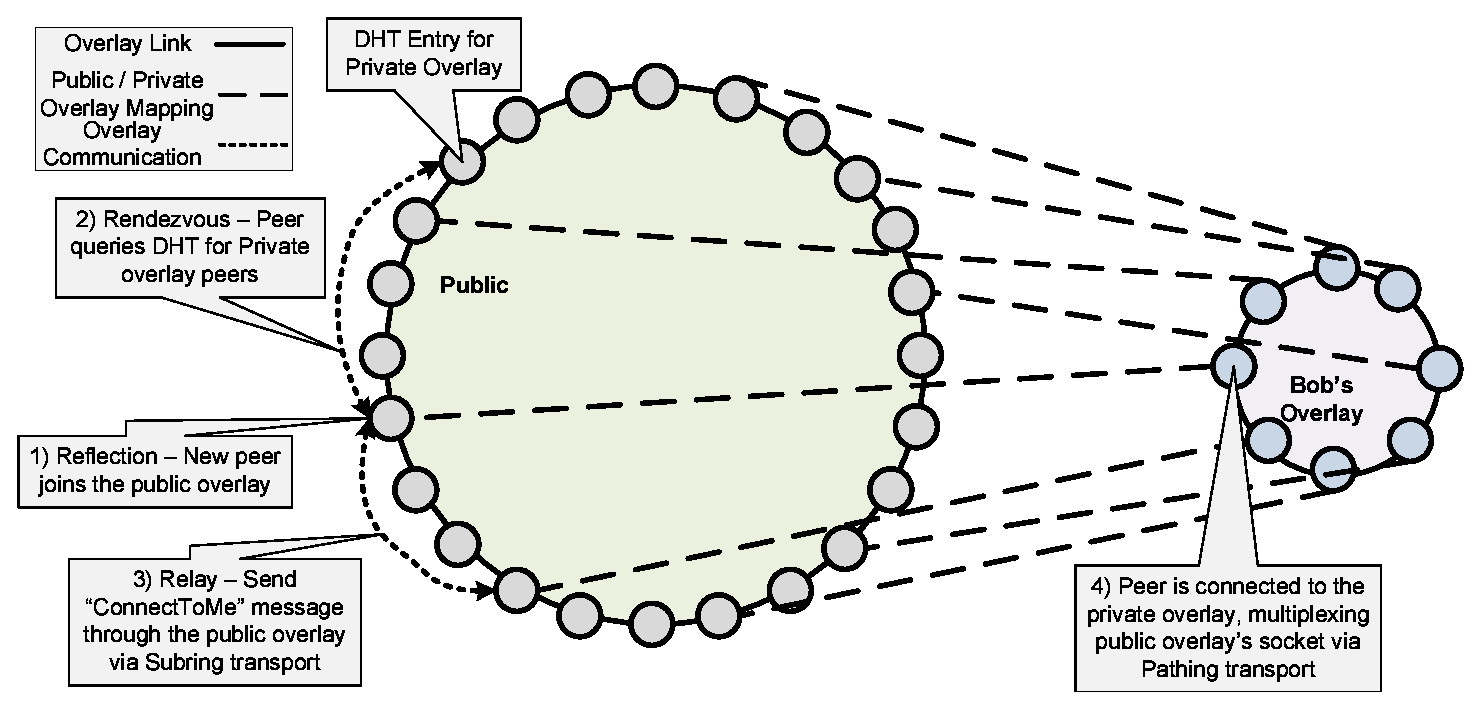
\epsfig{file=figs/bootstrap_brunet.eps, width=5.5in}
\caption{Bootstrapping a P2P system using Brunet.}
\label{fig:bootstrap_brunet}
\end{figure}
\end{center}

\subsection{Using XMPP}
\label{bs:xmpp_bootstrapping}

In addition to supporting recursive bootstrapping of private overlays, the
techniques described above can be extended to use a different public overlay,
an XMPP-based federation, to support the bootstrapping of private overlays.
The key features that make XMPP attractive are the distributed nature of the
federation and the openness of the protocol.  As of December 2009, there are
over 70 active XMPP servers in the XMPP Federation~\cite{xmpp_servers}.  These
include GoogleTalk, Jabber.org, and Live Journal Talk.

In XMPP, each user has a unique identifier of the form ``username@domain''.
Where the domain specifies the client's XMPP server and the username uniquely
identifies a single individual.  XMPP supports concurrent instances for each
user by appending a resource identifier to the user ID:
``username@domain/resource''.  A resource identifier can either be provided by
the client or generated by the server.  For users in the same domain, the
server forwards the message from source to destination.  When two users are in
different domains, the sender's server forwards the message to the receiver's
server, who then relays it to the receiver.

XMMP allows for sending arbitrary binary messages called ``IQ''.  While peer
relationships are maintained by the server, they are initiated between peers
using ``IQ''.  Once peers have established a connection or subscription, they
are informed through a ``Presence'' notification that the peer has come online,
this include the full user identifier.

The first form of reflection in XMPP is the unique client identifier.
Another is an IP reflection service available from some XMPP service providers
called ``Jingle''~\cite{jingle}.  ``Jingle'' uses ``IQ'' to determine available
STUN and TURN servers.  Fortunately, these services are provided free of charge
through GoogleTalk.  In Brunet, I extended the UDP transport to support
querying STUN servers to obtain and maintain and open an address mapping.  STUN
packets are easily distinguished from other packes as the first two bits are
set to 0 as well as a static cookie found in all messages.

In order to support the situation where two peers are unable to communicate
through the exchanged addresses, I have extended XMPP ``IQ'' as a transport to
support relaying.  Once peers has formed a connection through XMPP,
they are able to route connection information to each other and attempt to form
a direct connection.  In the case that this is unsuccessful, they are able to
fall back to this link as a means to transmit P2P data.  This approach also has
the benefit that, if a XMPP server does not support ``Jingle'', the two peers
can still form links with each other.  Since Brunet internally supports IP
reflection, eventually, if one of the peers in the system has a public address,
it will automatically assist the other peers into forming direct links with
each other.

Rendezvous uses a two step approach.  First peers advertise their use
of private overlay in the resource identifier.  The name is hashed to ensure
that the users complete identifier does not extend past 1,023 bytes, the
maximum length for these identifiers.  In addition, a cryptographically
generated random number is appended to the resource identifier to distinguish
between multiple instances of the users application in the same private
overlay.  Once a peer receives a presence notification from a remote peer and
the base components match, that is the hash of the service, the peer adds it to
a list of known online peers.  If the peer lacks connections, the system
broadcasts to that list a request for addresses.  The peers respond with a list
of addresses including UDP, TCP, and XMPP addresses, concluding rendezvous.

Ideally, peers would not need to create XMPP connections with each other; if
they are on a public address, the rendezvous phase alone will suffice.  When
peers do not have a public address, they can obtain a mapping through STUN,
then form an XMPP connection with each other, and finally perform simultaneous
connection attempts.  If NAT traversal fails, the peers can continue routing
through the XMPP connection.  Due to the abstractions employed by the transport
library, the additional support for XMPP-based bootstrapping required only an
additional 700 lines of code to Brunet and no modification to the core system.

\section{Evaluating Overlay Bootstrapping}
\label{bs:evaluations}

This section presents a qualitative evaluation of this system prototype
bootstrapping a small-scale network as well as some of the experiences in
deploying bootstrapping overlays.

\subsection{Deployment Experiments}

These experiments verify that the techniques work and determine expected
overheads in using Brunet and XMPP to bootstrap an overlay.  Rather than an
extensive experiment overly focused on overheads of Brunet and XMPP, this
experiment is primarily focused on the feasibility of forming small-scale
overlays among network-constrained peers.  The experiment represents 5 peers
desiring all-to-all direct connectivity, a feature transparently available to
them if they bootstrap into a private Brunet overlay. The experiments were run
on peers deployed on 5 distinct virtual machines.  Each virtual machine had its
own separate NAT, and thus peers were unable to communicate directly without
assistance.

The public Brunet overlay used in this experiment consisted of over 600 nodes
running on PlanetLab.  PlanetLab~\cite{planetlab} is a consortium of research
institutes sharing hundreds of globally distributed network and computing
resources.  GoogleTalk provided the XMPP overlay used in this experiment.
Though this experiment does not take into advantage the features of the XMPP
Federation, this aspect is presented in more detail in the next section
reviewing experiences deploying overlays using XMPP.

In the experiment, 5 P2P nodes were started simultaneously, while measuring the
time spent for reflection, rendezvous, reflection, and connection.  The results
are presented in Table~\ref{tab:results}.  For XMPP, these are translated as
follows:  reflection measures the time to obtain IP addresses from the STUN
server, rendezvous is the time to receive a presence notification, relaying is
the time to receive a message across XMPP, and connected is once all nodes in
the private overlay has all-to-all connectivity.  For Brunet, these are
translated as follows:  reflection measures the time to connect to the public
overlay, rendezvous is the time to query the DHT, relaying is the average time
to send a message across the overlay, and connected is the time until the
private overlay has all-to-all connectivity.  The results are highly correlated
to timeouts in Brunet, which employs a mixture of events and polling to
stabilize the overlay, as well as the latency between the client and
GoogleTalk.  As this was more of a qualitative experiment, the results are
clear: private overlays providing all-to-all connectivity among NATed nodes can
bootstrap within a very reasonable amount of time.

\begin{center}
\begin{table}
\caption{Time in seconds for various private overlay operations}
\begin{tabular*}{\textwidth}{@{\extracolsep{\fill}}
l
S[table-format=1.3,table-number-alignment=right]
S[table-format=1.3,table-number-alignment=right]
S[table-format=1.3,table-number-alignment=right]
S[table-format=2.2,table-number-alignment=right]
@{}
}

\hline & 
\multicolumn{1}{c}{Reflection} &
\multicolumn{1}{c}{Rendezvous} &
\multicolumn{1}{c}{Relaying} &
\multicolumn{1}{c}{Connected} \\ \hline
XMPP & .035 & .110 & .243 & 20.3 \\
Brunet & 3.05 & .330 & .533 & 23.22 \\ \hline
\end{tabular*}
\label{tab:results}
\end{table}
\end{center}

\subsection{Deployment Experiences}

Recently, Facebook announced that they would be supporting XMPP as a means to
connect to Facebook chat.  This was rather exciting and further motivated this
work, as Facebook has over 400 million active users, which would have made
their XMPP overlay, potentially, the largest free-to-join overlay.
Unfortunately, Facebook does not employ a traditional XMPP setup, instead it
provides a proxy into their chat network, preventing features like arbitrary
IQs and other forms of out-of-band messages to be exchanged between peers.
User identifiers are also translated, so a peer cannot obtain a remote peers
real identifier.  Thus there exists no out-of-band mechanism for rendezvous.
Peers could potentially send rendezvous messages through the in-band XMPP
messaging, but this may be viewed by most recipients as spam as it would arrive
as normal chat messages.  Unfortunately, the realization is that not all XMMP
servers, especially those unrelated to the Federation, support features
necessary to bootstrap.

During initial tests in verifying the workings of the XMPP code base, I
bootstrapped a private Brunet overlay on PlanetLab through various XMPP service
providers.  Unfortunately, some servers (GoogleTalk) ignored clients on
PlanetLab.  Another server crashed after 257 concurrent instances of the same
account logged in.  Because the provider had no contact information, I was
unable to ascertain the reason for the crash.  Though there did exist some
servers that had no trouble hosting over 600 concurrent instances running on
PlanetLab.

Once the system was running on PlanetLab, more tests were performed to
determine the ability to bootstrap across the XMPP Federation.  For this
purpose, several friendships, or subscriptions, were formed between users
across various XMPP service providers.  In the most evaluated case, a single
peer on GoogleTalk along with 600 peers on PlanetLab system using
\textit{jabber.rootbash.com}, the GoogleTalk peer would not always receive
presence notifications for all peers online, though always would receive some.
When a peer began the relaying mechanism, it would broadcast to every peer from
whom it received a presence notification.  When performing this between
GoogleTalk and \textit{rootbash}, the GoogleTalk peer would not receive a
response.  Though in reducing the broadcast to a random selection of 10 peers,
every 10 seconds until the GoogleTalk peer was connected, the peer received
responses.  The behavior indicates that the XMPP servers may have been
filtering to prevent denial of service attacks.

Peers on the same XMPP server seem to be connected very quickly, though peers
on different services can take significantly longer.  For example, when
bootstrapping a single peer from GoogleTalk into the \textit{rootbash} system,
it always took 1 minute for the node to become fully connected to the private
overlay.  When the peer used \textit{rootbash}, the peer always connected
within 30 seconds.  It seems as if the communication between XMPP servers was
being delayed for some reason.  The same behavior was not experienced, when
chatting between the two peers.

\begin{center}
\singlespacing{
\footnotesize{
\begin{longtable}{p{.85in}p{1.5in}p{1.2in}p{1.05in}p{1.05in}}

\caption{Public and research overlays.} \\

\hline & Description & Reflection & Rendezvous & Relay \\ \hline
\endfirsthead

\multicolumn{5}{l}{\normalsize{Table \ref{tab:overlays}. Continued}}\\
\hline & Description & Reflection & Rendezvous & Relay \\ \hline
\endhead

BitTorrent &
Default BitTorrent implementations rely on a centralized tracker to provide the
initial bootstrapping.  Peers can establish new connections through information
obtained from established connections.  This relegates the tracker as a means
of monitoring the state of the file distribution.  BitTorrent specifies a
protocol, though each client may support additional features not covered by the
protocol.
&
The current specification does not support NAT traversal, though future
versions may potentially use UDP NAT traversal.  At which point, BitTorrent may
support a reflection service.
&
Peers can register as seeds to the same file hash, thus their IP address will
be stored with the tracker.
&
Peers receive each other's IP addresses from the tracker, there is no inherent
relaying.
\\ 
Gnutella &
Gnutella is a large-scale unstructured overlay with over a million peers;
primarily, it is used for file sharing.  Gnutella consists of a couple
hundred thousand ultra (super) peers to provide reliability to the overlay.
Gnutella is free-to-join and requires no registration to use.
&
Work in progress.  Peers attempt to connect to a sharer's resource, though a
"Push" notification reverses this behavior.  Thus a peer behind a NAT can
share with a peer on a public address.
&
Peers can perform broadcast searches with TTL up to 2; when networks consist of
millions of peers, small overlays will most likely not be able to discover each
other.
&
Not explicitly, could potentially utilize ping messages to exchange messages.
\\ 
Skype &
Skype is a large-scale unstructured overlay, consisting of over a million
active peers, and primarily used for voice over P2P communication.  Skype, like
Gnutella, also has super peers, though the owners of Skype provide
authentication and bootstrap servers.  Though Skype is free-to-join, it
requires registration to use.
&
Skype APIs provide no means for reflection.
&
Skype supports applications, or add-ons, which can used to transparently
broadcast queries to a users friend to determine if the peer has the
application installed.  Thus Skype does support rendezvous.
&
Skype applications are allowed to route messages via the Skype overlay, but
because Skype lacks reflection, all communication must traverse the Skype
overlay.
\\ 
XMPP &
XMPP consists of a federation of distributed servers.  Peers must register an
account with a server, though registration can be done through XMPP APIs without
user interaction.  XMPP is not a traditional P2P system, though it has some P2P
features.  XMPP servers on distinct servers are able to communicate with each
other.  Links between servers are created based upon client demand.  During link
creation, servers exchange XMPP Federation signed certificates.
&
While not provided by all XMPP servers, there exist extensions for NAT
traversal.  GoogleTalk, for example, provides both STUN and TURN servers.
&
Similar to Skype, XMPP friends can broadcast queries to each other to find
other peers using the same P2P service.  Thus XMPP supports rendezvous.
&
The XMPP specification allows peers to exchange arbitrary out-of-band
communication with each other.  Most servers support this behavior, even
when sent across the Federation.  Thus XMPP supports relaying.
\\ 
Kademlia~\cite{kademlia} &
There exists two popular Kademlia systems, one used by many BitTorrent systems,
Kad, and the other used by Gnutella, called Mojito.  Kademlia implements an
iterative structured overlays, where peers query each other directly when
searching the overlay.  Thus all resources of a Kademlia overlay must have
a publicly addressable network endpoint.
&
Existing implementations of Kademlia do not support mechanims for peers to
determine their network identity.
&
Peers can use the DHT as a rendezvous service, storing their connectivity
information in the DHT at key location:  $hash(SERVICE)$.
&
An iterative structured overlay has no support for relaying messages.
\\ 
OpenDHT~\cite{opendht} &
OpenDHT is a recently decommissioned DHT running on PlanetLab.  OpenDHT is
built using Bamboo, a Pastry-like protocol~\cite{pastry}.  Pastry implements
recursive routing, peers route messages through the overlay.
&
Existing implementations of Bamboo and Pastry do not support mechanims for
peers to determine their network identity.  Though this is ongoing work.
&
Peers can use the DHT as a rendezvous service, storing their connectivity
information in the DHT at key location:  $hash(SERVICE)$.
&
Because Pastry uses recursive routing, it can be used as a relay.  Furthermore,
extensions to Pastry have enabled explicit relays called virtual
connections~\cite{epost}.
\\ 
Brunet~\cite{brunet} &
Brunet like OpenDHT is a freely available DHT running on PlanetLab, though
still in active development.  Brunet creates a Symphony~\cite{symphony} overlay
using recursive routing.
&
Brunet supports inherent reflection services, when a peer forms a connection
with a remote peer, the peers exchange their view of each other.
&
Peers can use the DHT as a rendezvous service, storing their connectivity
information in the DHT at key location:  $hash(SERVICE)$.
&
Like Pastry, Brunet supports recursive routing and relays called
tunnels~\cite{hpdc08_0}.
\\ 
\label{tab:overlays}
\end{longtable}}}
\end{center}

